\section*{Reproducibility}

Hollmann and colleagues evaluated TabPFN on 29 classification and 28 regression datasets with up to 10,000 rows, 500 features and 10 classes, using ten seeds with a 90/10 train/test split, baselines tuned by random search for between 30 seconds and four hours, scores normalised within each dataset (best method 1, worst 0), and a GPU for TabPFN.\citep{hollmann2025accurate} We did not repeat that protocol. We re-ran TabPFN on seven of its classification datasets (ada, australian, blood-transfusion, car, churn, cmc and credit-g), reporting raw ROC AUC on one stratified split per dataset that held out 15\% of rows, and compared TabPFN with CatBoost, XGBoost, LightGBM, random forest, logistic regression and AutoGluon, all without hyperparameter tuning. Baseline runs for ada did not complete, leaving six datasets for the comparison.

The direction of the central claim reproduced (Fig.~\ref{fig:reproduction}a,b). TabPFN had the highest mean test ROC AUC, 0.877, followed by CatBoost at 0.873, XGBoost at 0.863 and AutoGluon at 0.861; logistic regression reached 0.797. TabPFN was best or tied for best on four of six datasets, second on credit-g and fourth on churn. These raw ROC AUC values are not comparable with the original's normalised scores, which were 0.939 for default TabPFN and 0.752 for default CatBoost on classification.\citep{hollmann2025accurate} With six datasets and one split each, and baselines that were not tuned, our margins confirm the direction of the original finding and not its size.

We then compared generations under a common protocol with training sets capped at 1,024 rows (Fig.~\ref{fig:reproduction}c). On the six datasets where every model completed (TabPFN v3 failed on ada in this run), mean ROC AUC was 0.856 for TabPFN v1, 0.862 for v2, 0.863 for v2.5, 0.857 for v2.6, 0.861 for v3 and 0.859 for TabFM. On small public benchmarks, then, successive generations and an independently developed foundation model behave almost interchangeably. Rankings in large benchmarks depend on tuning budgets, validation design and ensembling,\citep{erickson2025tabarena,qu2025tabicl} so we compare generations only under this one protocol and do not rank them in general.

\begin{figure}[t]
\centering
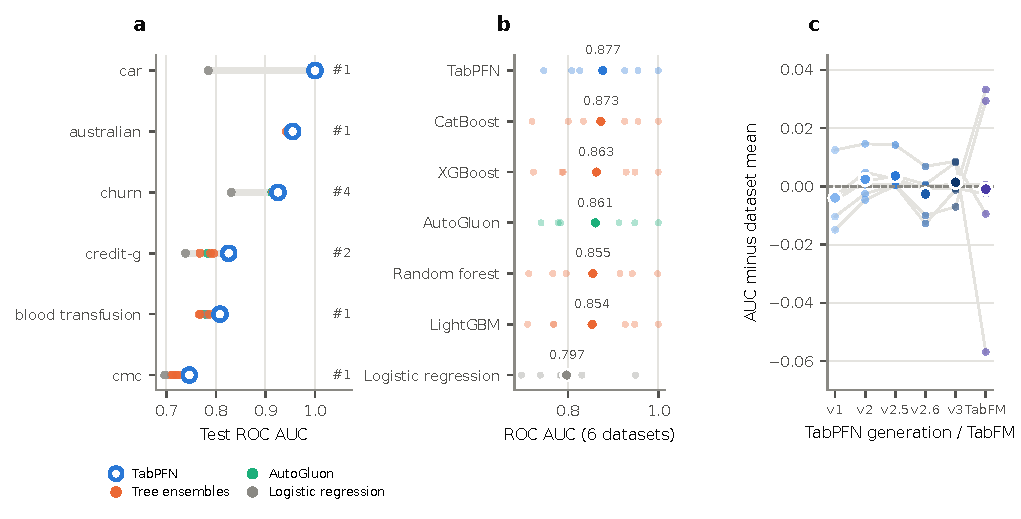
\includegraphics[width=\linewidth,height=0.64\textheight,keepaspectratio]{figures/reusability/fig2_reproduction.pdf}
\caption{\textbf{The direction of TabPFN's benchmark advantage reproduces on its own datasets.} \textbf{a}, TabPFN against six baselines: test ROC AUC of TabPFN (open circle) and of tree ensembles, AutoGluon and logistic regression (filled points) on six benchmark datasets. The grey bar spans the baselines, and the number on the right is TabPFN's rank on that dataset (ties share a rank). \textbf{b}, Mean test ROC AUC of each model over the six datasets (large point, value above) with per-dataset values (small points). \textbf{c}, Four TabPFN generations and TabFM under a common protocol with training capped at 1,024 rows: ROC AUC relative to each dataset's mean across these six models (lines join datasets; large points are means). Mean ROC AUC over the six datasets was 0.856 (v1), 0.862 (v2), 0.863 (v2.5), 0.857 (v2.6), 0.861 (v3) and 0.859 (TabFM). One stratified split per dataset.}
\label{fig:reproduction}
\end{figure}
